\documentclass[8.01x]{subfiles}
\begin{document}

\chapter{Week 1: Homework 1}

\section{Problem 1: Decomposing vectors}

``Consider two vectors in the xy-plane as shown.

\begin{center}
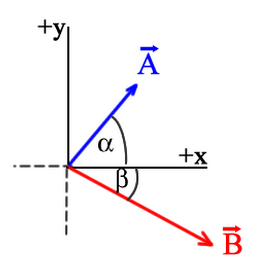
\includegraphics[scale=0.8]{Graphics/h1p1}
\end{center}

Vector $\vec{A}$, in the first quadrant, has a magnitude $|\vec{A}| = 2.0$ and is at an angle $\alpha = \ang{40}$ with respect to the positive x-axis. Vector $\vec{B}$, in the fourth quadrant, has a magnitude $|\vec{B}| = 1.5$ and is at an angle $\beta = \ang{20.0}$ with respect to the positive x-axis.

Find the x and y components of the vectors $\vec{A}$ and $\vec{B}$.''

Well, this ought to be fairly simple. First, let's consider what sort of values we expect. $\alpha$ is in the first quadrant that is, angled upwards and to the right. That means $A_x > 0$ and $A_y > 0$.\\
We could use the formulas listed in the first part of these notes, or simply re-derive them from the basic trig definitions. I prefer the latter route, since it can be done in a few seconds once you're comfortable with it, and it means you can't remember them the wrong way. (Unless you misremember everything central to trigonometry!)

$A_x$ is the adjacent side to $\alpha$, while $\vec{A}$ is the hypotenuse, and $A_y$ is the opposite. Using trig definitions, we find

\begin{equation}
\sin \alpha = \frac{A_y}{|\vec{A}|}
\end{equation}
\begin{equation}
A_y = |\vec{A}| \sin \alpha
\end{equation}

\begin{equation}
\cos \alpha = \frac{A_x}{|\vec{A}|}
\end{equation}
\begin{equation}
A_x = |\vec{A}| \cos \alpha
\end{equation}

The same relations hold for $\beta$ and $\vec{B}$ as well, of course, so we just need to enter these answers into the form (and convert the degree values to radians inside the trig functions), and we're done!

\section{Problem 2: Catching up}

``During a track event two runners, Mary, and Alice, round the last turn and head into the final stretch with Mary a distance $d = 3.0$ m in front of Alice. They are both running with the same speed of $v_0 = 7.0$ m/s. When the finish line is a distance $L = 45.0$ m away from Alice, Alice accelerates at $a_A = 1.5\text{ m/s}^2$ until she catches up to Mary. Alice then continues at a constant speed until she reaches the finish line.

\begin{center}
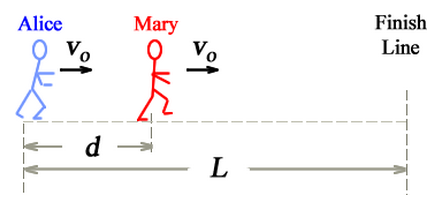
\includegraphics[scale=0.8]{Graphics/h1p2}
\end{center}

(a) How long (in s) did it take Alice to catch up with Mary?''

First up, we need to choose a reference frame to work in. I considered choosing Mary's reference frame, so that she is seen as stationary, but that would probably just cause problems in some aspects of the problem.\\
I'll therefore choose the simple one, where the track and the finish line are stationary.

Since there are five sub-question, let's set up some equations. We know the initial position of each runner (we'll call Alice's position 0, and therefore Mary's initial position is $d$), initial velocity, and acceleration.

For Alice:
\begin{align}
x_A(t) = v_0 t + \frac{3}{4} t^2\\
v_A(t) = v_0 + 1.5 t
\end{align}
(Alice's acceleration is due to the \SI{1.5}{m/s^2} times the one-half present in the formula.)

And for Mary:
\begin{align}
x_M(t) &= d + v_0 t\\
v_M(t) &= v_0
\end{align}

So, let's restate the question:
``(a) How long (in s) did it take Alice to catch up with Mary?''

We set their position equations equal, and solve for $t$:

\begin{align}
\frac{3}{4} t^2 = d\\
t^2 = \frac{4}{3} d\\
t = +\sqrt{\frac{4d}{3}} = \SI{2}{s}
\end{align}

``(b) How far (in m) did Alice still have to run when she just caught up to Mary?''

It took 2 seconds exactly, so Mary must have moved 14 meters (2 seconds, 7 m/s) in that time, to position $d + \SI{14}{m}$.\\
The distance remaining is $L - d - \SI{14}{m} = \SI{28}{m}$.

``(c) How long (in s) did Alice take to reach the finish line after she just caught up to Mary?''

Keep in mind that she stopped accelerating when she passed, so her velocity is now a constant again. She started out at 7 m/s and accelerated at \SI{1.5}{m/s^2} for 2 seconds, so her velocity is now \SI{10}{m/s}. The answer is the distance remaining divided by her velocity, so the answer is

\begin{equation}
\text{time taken} = \frac{L - d - \SI{14}{m}}{\SI{10}{m/s}} = \SI{2.8}{s}
\end{equation}

``Mary starts to accelerate when Alice just catches up to her, and accelerates all the way to the finish line and crosses the line exactly when Alice does. Assume Mary's acceleration is constant.\\
(d) What is Mary's acceleration (in $\text{m/s}^2$)?''

To sum up where we're at: Mary is still running at 7 m/s, with 28 meters left to go. Alice is running at 10 m/s, also with 28 meters left to go (meaning she will get there in 2.8 seconds).\\
Mary must now accelerate such that $x_M(t) = L$ at $t = \SI{2.8}{s}$ (we reset the current time to $t=0$ for simplicity).

Mary's new position equation is

\begin{equation}
x_M(t) = (L - \SI{28}{m}) + v_0 t + \frac{1}{2} a t^2
\end{equation}

We need that it to be equal to $L$ at $t = \SI{2.8}{s}$ as mentioned, so we substitute the values for $t = \SI{2.8}{s}$ and $v_0 = \SI{7}{m/s}$ in, set it equal, and solve for $a$:

\begin{align}
(L - \SI{28}{m}) + (\SI{7}{m/s})(\SI{2.8}{s}) + \frac{1}{2}\ a\ (\SI{2.8}{s})^2 = L\\
- \SI{28}{m} + \SI{19.6}{m} + \SI{3.92}{s^2} \cdot a = 0\\
\SI{3.92}{s^2} \cdot a = \SI{28}{m} - \SI{19.6}{m}\\
a = \frac{\SI{28}{m} - \SI{19.6}{m}}{\SI{3.92}{s^2}} \approx \SI{2.14}{m/s^2}
\end{align}

``(e) What is Mary's velocity at the finish line (in m/s)?''

That would be given by her old velocity, 7 m/s, plus the acceleration multiplied by the time accelerated (2.8 seconds):

\begin{equation}
v_{M_{final}} = \SI{7}{m/s} + \SI{2.14}{m/s^2} \cdot \SI{2.8}{s} \approx \SI{13}{m/s}
\end{equation}

\section{Problem 3: Speeding ticket}

This problem was removed from the grading, i.e. assigned 0 points, after there had been some trouble with it. The problem is supposed to be fixed now, however, so I will attempt it.

``A motorist traveling with constant speed of $v_c = 18.0$ m/s passes a school-crossing corner, where the speed limit is 10 m/s. Just as the motorist passes, a police officer on a motorcycle stopped at the corner starts off in pursuit. The officer accelerates from rest at $a_m = \SI{3.00}{m/s^2}$ until reaching a speed of 30.0 m/s. The officer then slows down at a constant rate until coming alongside the car at x = 270.0 m.\\
Consider a coordinate system with origin at the school-crossing corner, $x = 0$, and the +x-axis in the direction of the car's motion.

(a) How long does it take for the motorcycle to catch up with the car (in s)?''

Okay. The car moves at a constant velocity, so that part is easy. Now, as for the offices, he takes 10 seconds to accelerate to his top speed. During that time, his new position is

\begin{align}
x_m(t=10) &= x_0 + v_0 t + \frac{1}{2} a t^2 = \frac{1}{2} (\SI{3}{m/s^2}) (\SI{10}{s})^2\\
          &= \SI{150}{m} \text{ (answers question c)}
\end{align}

As mentioned above, this also  answers part (c): ``(c) How far (in m) is the motorcycle from the corner when switching from speeding up to slowing down?''

In fact, I think the next question that should be answered is (d), not (a), so let's see.

``(d) How far (in m) is the motorcycle from the car when switching from speeding up to slowing down?''

We don't really need to write down the position equation here, as it's a bit too simple: $x = \SI{18.0}{m/s} \cdot \SI{10}{s} = \SI{180}{m}$. Since the motorcycle is 150 m from the corner, the answer here must be 30 m.

So, we are now at: motorist at $x = 180$ m at 18.0 m/s, cop at $x = 150$ m at 30.0 m/s. The cop must slow down with constant acceleration so that he hits $x = 270$ m at the same time as the motorist. At the motorists' speed, that happens at

\begin{equation}
t = \SI{10}{s} + \frac{\SI{270}{m} - \SI{180}{m}}{\SI{18.0}{m/s}} = \SI{15}{s}
\end{equation}

... where 10 seconds is the time that has already passed. Alternatively, we could simply take the 270 meters divided by the velocity to find the same result. This answers question (a). Back to (e):

All in all, we set up a new equation for the cop. $x_0 = \SI{150}{m}$, $v_0 = \SI{30.0}{m/s}$, and $a$ is our unknown. The position equation must equal 270 m at $t = \SI{5}{s}$ -- we reset $t$ to start over from the instant where the above parameters are true:

\begin{align}
\SI{150}{m} + (\SI{30.0}{m/s})(\SI{5}{s}) + \frac{1}{2} a (\SI{5}{s})^2 = \SI{270}{m}\\
\frac{1}{2} a (\SI{5}{s})^2 = \SI{-30}{m}\\
a (\SI{25}{s^2}) = \SI{-60}{m}\\
a  = \frac{\SI{-60}{m}}{\SI{25}{s^2}} = \SI{-2.4}{m/s^2}
\end{align}

\section{Problem 4: Position, velocity and acceleration}

``An object is moving along a straight line parallel to the x-axis. Its position as a function of time is given by:\\
$x(t) = \SI{30}{m} - (\SI{21}{m/s}) t + (\SI{3}{m/s^2}) t^2$\\
where the position x is in meters and the time t is in seconds.

(a) What is the object's velocity at $t = 0$ s, 2 s, and 5 s?''

We take the derivative of the above equation, and end up with

\begin{equation}
v(t) = - \SI{21}{m/s} + (\SI{6}{m/s^2}) t
\end{equation}

All we need to do now is plug in the values for $t$.

``(b) What is the object's acceleration at $t = 0$ s, 2 s, and 5 s?''

We take the derivative of $v(t)$ above:

\begin{equation}
a(t) = \SI{6}{m/s^2}
\end{equation}

We don't even need to plug in values here - the answer is $\SI{6}{m/s^2}$ for all three cases.

``(c) At what time T is the object's velocity zero?''

We set $v(t) = 0$ and solve for $t$:

\begin{align}
- \SI{21}{m/s} + (\SI{6}{m/s^2}) t = 0\\
t = \frac{\SI{21}{m/s}}{(\SI{6}{m/s^2})}\\
t = \SI{3.5}{s}
\end{align}

``What is the object's position when its velocity is zero?''

We plug $t = \SI{3.5}{s}$ into $x(t)$ and we're done. Note that the answer (in my case, at least) is negative.

``(d) What is the average velocity between $t_1 = \SI{1.0}{s}$ and $t_2 = \SI{3.5}{s}$?''

With a constant acceleration, as here, we can calculate the average simply by averaging between the velocities at $t_1$ and $t_2$.

\begin{equation}
v_{t_1 t_2 avg} = \frac{v(\SI{1.0}{s}) + v(\SI{3.5}{s})}{2} = \frac{\SI{-15}{m/s} + \SI{0}{m/s}}{2} = \SI{-7.5}{m/s}
\end{equation}

``(e) What is the object's average velocity between $t_1 = \SI{0}{s}$ and $t_2 = \SI{7.0}{s}$?''

Same deal as above.

\begin{equation}
v_{t_1 t_2 avg} = \frac{v(\SI{0}{s}) + v(\SI{7}{s})}{2} = \frac{\SI{-21}{m/s} + \SI{21}{m/s}}{2} = \SI{0}{m/s}
\end{equation}

``(e) What is the object's average speed between $t_1 = \SI{0}{s}$ and $t_2 = \SI{7.0}{s}$?''

Aha! Keep in mind that speed and velocity are \emph{not} the same in physics! Here, because the object has reversed, the average speed will be greater than the average velocity. How do we calculate the speed, though?

Well, we know that the object stops at $t = \SI{3.5}{s}$, from (c) above. We can also show very simply that it reverses direction at that point.
We can find the average speed as the total distance traveled, divided by the 7 seconds.\\
The first part of the distance is $|x(\SI{3.5}{s}) - x(\SI{0}{s})|$, and the second part is $|x(\SI{7}{s}) - x(\SI{3.5}{s})|$.

\begin{equation}
\text{avg speed} = \frac{|x(\SI{3.5}{s}) - x(\SI{0}{s})| + |x(\SI{7}{s}) - x(\SI{3.5}{s})|}{\SI{7}{s}} = \SI{10.5}{m/s}
\end{equation}

That wasn't very pretty, but it worked.

``(g) At what time $t_3$ does the object reverse its direction?''

That was answered in passing above: at $t_3 = \SI{3.5}{s}$.

\section{Problem 5: One-dimensional kinematics}

``Two stones are released from rest at a certain height, but at different times. When answering the following questions, ignore air drag.

(a) Will the difference between their speeds increase, decrease, or stay the same?''

The two will have the same acceleration ($-g \approx \SI{-9.8}{m/s^2}$), of course, but they are released at different times. The one released first will have fallen for a longer time, all the way until it hits the ground.\\
The acceleration causes a linear change in the velocity, adding $\SI{-9.8}{m/s}$ every second, to both stones.\\
If one is released at $t=0$ and the other at $t = \SI{1}{s}$, at the instant where the second stone is released, one stands still and one moves at $\SI{-9.8}{m/s^2}$. Ten seconds later, one moves with $\SI{-107.8}{m/s^2}$ and the other at $\SI{-98}{m/s^2}$.

So indeed, the difference is constant, as we expected from the third sentence above.

``(b) Will their separation distance increase, decrease, or stay the same?''

Now this is a bit interesting. When something falls in a gravitational field, its velocity increases all the time (as long as we ignore air drag, which creates an upper limit to the velocity). In the above example, if the separation begins at $\SI{4.9}{m}$ ($\displaystyle x(t) = \frac{\SI{-9.8}{m/s^2}}{2} t^2$), but after another 10 seconds, the separation is much greater. Thus the answer is that it increases.

``(c) Will the time interval between the instants at which they hit the ground be smaller than, equal to, or larger than the time interval between the instants of their release?''

This is something I expect could get a bit tricky if we get into the equations, but it's obvious that the answer \emph{must} be ``equal''. Both have the position function $\displaystyle x(t) = \frac{\SI{-9.8}{m/s^2}}{2} t^2$, so they must fall in the same trajectory, taking the same time to fall. Therefore, if we release them at the same time, they must hit the ground at the same time. If we release them one second apart, they must hit the ground one second apart, etc.

\section{Problem 6: Elevator}

\begin{center}
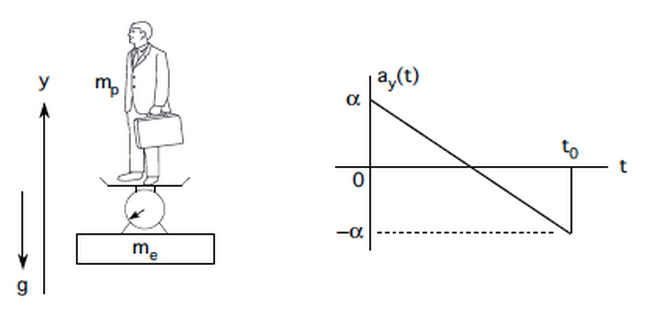
\includegraphics[scale=0.8]{Graphics/h1p6}
\end{center}

``A person of mass $m_p$ stands on a scale in an elevator of mass $m_e$. The scale reads the magnitude of the force $F$ exerted on it from above in a downward direction. Starting at rest at $t = 0$ the elevator moves upward, coming to rest again at time $t = t_0$. The downward acceleration of gravity is $g$ . The acceleration of the elevator during this period is shown graphically above and is given analytically by\\
$\displaystyle a_y(t) = \alpha - \frac{2\alpha}{t_0} t$\\
a) Find the maximum speed of the elevator. Express your answer in terms of $\alpha$ and $t_0$.\\
b) Find the total distance traveled by the elevator.''

Uh, okay. Honestly, I'm a bit confused -- it doesn't appear as if the man, his mass, the scale, the mass of the elevator or $g$ matter whatsoever! These questions don't tend to include information to make them appear harder than they are, though.\\
I suppose I'll get started by ignoring them and see what happens.

The elevator is stationary to begin with. That means we can say not only $y_0 = 0$, but also $v_0 = 0$. However, as nice as it would be, we cannot use $v(t) = a_y t$, since the acceleration is not constant. We must integrate the acceleration. Note, however, that the acceleration starts at $\alpha$, and progresses all the way to $-\alpha$, and that the graph is symmetric around the middle. The integral of the entire interval is zero. We want the maximum speed, which should happen just as it reverses, so at $t_0/2$.

\begin{align}
s_{max} &= \int_0^{t_0/2} a_y(t) dt = \int_0^{t_0/2} \left( \alpha - \frac{2\alpha}{t_0} t \right) dt = \left[\alpha t - \frac{\alpha}{t_0} t^2\right]_{t=0}^{t=t_0/2}\\
        &= \left(\alpha \frac{t_0}{2} - \frac{\alpha}{t_0} \frac{t_0^2}{4} \right) - (0 - 0)\\
        &= \alpha \left(\frac{t_0}{2} - \frac{t_0}{4} \right)\\
        &= \frac{\alpha t_0}{4}
\end{align}

That indeed works.

``b) Find the total distance traveled by the elevator, $y(t_0)$.''

Let's begin by finding the velocity function (as an indefinite integral).

\begin{align}
v(t) &= \int \left( \alpha - \frac{2\alpha}{t_0} t \right) dt  = \alpha t - \frac{2\alpha}{t_0} \frac{t^2}{2}\\
     &= \alpha \left( t - \frac{t^2}{t_0} \right)
\end{align}

We can forget about the $+ C$. The constant here would be $v_0$, and we know that to be zero.

We now know the velocity at any point between $t = 0$ and $t = t_0$, but that doesn't help us much yet -- it's not constant, so we need to integrate again, to find the position function.

\begin{align}
y(t) &= \int \alpha \left( t - \frac{t^2}{t_0} \right) dt\\
     &= \alpha\left( \frac{t^2}{2} - \frac{t^3}{3t_0} \right)\\
\end{align}

We substitute $t = t_0$:

\begin{align}
y(t_0) &= \alpha\left( \frac{t_0^2}{2} - \frac{t_0^3}{3t_0} \right)\\
       &= \alpha t_0^2 \left( \frac{1}{2} - \frac{1}{3} \right)\\
       &= \frac{\alpha t_0^2}{6}
\end{align}

... and we're done, indeed by ignoring the majority of the information given. Strange problem.

\section{Problem 7: Position, velocity, and acceleration in 3D}

``A particle is moving in three dimensions. Its position vector, $\vec{r}$, is given by\\
$\vec{r}(t) = (6 - 2t)\hat{x} + (3 + 4t - 6t^2)\hat{y} - (1 + 3t - 2t^2)\hat{z}$

Distances are in meters, and the time, $t$, in seconds.\\
(a) What are the components of the velocity vector (in m/s) $\vec{v}$  at $t = +3$?''

As usual, we need to take the derivative. We calculate the derivative of each dimension on its own, and sum up the results.

\begin{align}
\vec{v} &= -2\hat{x} + (4 - 12t)\hat{y} - (3 - 4t)\hat{z} \label{eq:h1p7_velocity}\\
v_x &= -2\\
v_y &= 4 - 12 \cdot 3 = -32\\
v_z &= -3 + 4 \cdot 3 = 9
\end{align}

``(b) What is the speed (in m/s) at $t =+3$?''

Speed at an instant is simply the magnitude of the velocity (as they point out when they also ask for $|\vec{v}|$).

\begin{equation}
|\vec{v}| = \sqrt{v_x^2 + v_y^2 + v_z^2} = \sqrt{(-2)^2 + (-32)^2 + 9^2} \approx \SI{33.3}{m/s}
\end{equation}

``(c) What are the components of the acceleration vector $\vec{a}$ (in $\text{m/s}^2$) at $t = +3$?''

We calculate the derivative of the velocity, i.e. equation \eqref{eq:h1p7_velocity}.

\begin{equation}
\vec{a} = -12 \hat{y} + 4\hat{z}
\end{equation}

``(d) What is the magnitude of the acceleration vector $\vec{a}$ (in $\text{m/s}^2$) at $t = +3$?''

We do what we did for the velocity vector.

\begin{equation}
|\vec{a}| = \sqrt{(-12)^2 + 4^2} \approx \SI{12.65}{m/s^2}
\end{equation}

\section{Problem 8: Vertical collision}

``Mary wants to throw a can straight up into the air and then hit it with a second can. She wants the collision to occur at height $h = 5.0$ m above the throw point. In addition, she knows that she needs $t_1 = \SI{4.0}{s}$ between successive throws. Assuming that she throws both cans with the same speed. Take $g$ to be \SI{9.81}{m/s^2}.

(a) How long it takes (in s) after the first can has been thrown into the air for the two cans to collide?\\
(b) Find the initial speed of the cans (in m/s).''

The grammar in the question text might need a bit of a double-check (I spot two errors, and one slightly confusing statement)! Re-stated, I read it as something like this:\\
She throws the two cans up in into the air, with the same unknown velocity $v_0$, 4 seconds apart (one at $t = 0$, one at $t = \SI{4.0}{s}$). How long after $t = 0$ do the cans collide, assuming it happens at $h = \SI{5.0}{m}$?

In these equations, increasing $y$ is defined as upwards. Therefore, gravitational acceleration is $-g$. I choose to define $y_0 = 0$, since that simplifies things. (Rather, choosing anything else would needlessly complicate things.)

\begin{align}
 y_1(t) &= v_0 t - \frac{1}{2} g t^2\\
 y_2(t) &= v_0 t' - \frac{1}{2} g t'^2\\
\end{align}

... where $t' = t - \SI{4.0}{s}$.
Let's set $y_1 = y_2$ and see what happens.

\begin{align}
v_0 t - \frac{1}{2} g t^2 &= v_0 t' - \frac{1}{2} g t'^2\\
v_0 t - \frac{1}{2} g t^2 &= v_0 (t - 4) - \frac{1}{2} g (t - 4)^2\\
v_0 t - \frac{1}{2} g t^2 &= v_0 t - 4 v_0 - \frac{1}{2} g (t^2 -8t + 16)\\
t^2 &= \frac{- 4 v_0}{- \frac{1}{2} g} + (t^2 -8t + 16)
\end{align}

We simplify this into a linear equation, and solve it.

\begin{align}
0 &= \frac{8v_0}{g} + -8t + 16\\
t &= \frac{v_0}{g} + 2
\end{align}

Hmm, we're a bit stuck here, since $v_0$ is an unknown. Let's try to add another equation to the mix and see if we can solve for that. The \emph{next} sub-question is about finding $v_0$.

We do have another piece of information, that we have not used: $y_1(t) = y_2(t) = h$, for the time $t$ where they collide. We have not used $h$ yet.

\begin{align}
v_0 t - \frac{1}{2} g t^2 = h\\
v_0 t = h + \frac{1}{2} g t^2\\
v_0 = \frac{h}{t} + \frac{1}{2} g t \label{h1p8:v0}
\end{align}

Combine the two equations and finally solve for $t$:

\begin{align}
t &= \frac{1}{g} \left(\frac{h}{t} + \frac{1}{2} g t\right) + 2\\
t &= \frac{h}{gt} + \frac{1}{2} t + 2\\
\frac{t}{2} &= \frac{h}{gt} + 2
\end{align}

Multiply both sides by $2t$ and we finally have a quadratic to solve:

\begin{equation}
t^2 - 4t - \frac{2h}{g} = 0
\end{equation}
\begin{equation}
t = \frac{4 \pm \sqrt{(-4)^2 + \frac{8h}{g}}}{2} = \frac{4 \pm 4.48}{2} = \SI{4.24}{s}
\end{equation}

... neglecting the other solution, which is negative and therefore not applicable. Our equations are only valid from $t = 0$.

``(b) Find the initial speed of the cans (in m/s).''

We have that in equation \eqref{h1p8:v0}, so we plug in the values:

\begin{equation}
v_0 = \frac{\SI{5}{m}}{\SI{4.24}{s}} + \frac{1}{2} (\SI{9.81}{m/s^2}) (\SI{4.24}{s}) \approx \SI{22.0}{m/s}
\end{equation}

\section{Problem 9: Vector operations}

Since these are essentially just multiplication, I didn't bother to take notes for them. Cross products can be a bit painful when using components, but as far as I know, using calculators is allowed for this course.\\
I wouldn't recommend doing that unless you feel certain that you could also do it \emph{without} a calculator, however.

\section{Problem 10: Perpendicular vectors}

``The vectors $\vec{A} = 1 \hat{x} - 2 \hat{y}$ and $\vec{B} = -4 \hat{x} + a \hat{y} - 2\hat{z}$ are perpendicular to each other. What is the value of a?''

Honestly, I looked up a small hint for this one: that the dot product of two perpendicular vectors has a special property. That was enough to see the solution: the dot product will always be zero. We can set the dot product equal to zero and solve for $a$. Simple!

\begin{equation}
\vec{A} \cdot \vec{B} = A_x B_x + A_y B_y + A_z B_z
\end{equation}

\begin{align}
(1)(-4) + (-2)(a) + (0)(-2) = 0\\
-4 - 2a = 0\\
a = -2
\end{align}

Dead simple once you realize how to solve it.

That's it for this week!

\end{document}